\documentclass{beamer}
\usepackage[utf8]{inputenc}

\usetheme{Madrid}
\usecolortheme{default}
\useinnertheme{circles}

\definecolor{Logo1}{rgb}{0.208, 0.2865, 0.373}
\definecolor{Logo2}{rgb}{0.000, 0.674, 0.863}

\setbeamercolor*{palette primary}{bg=Logo1, fg=white}
\setbeamercolor*{palette secondary}{bg=Logo2, fg=white}
\setbeamercolor*{palette tertiary}{bg=white, fg=Logo1}
\setbeamercolor*{palette quaternary}{bg=Logo1,fg=white}
\setbeamercolor{structure}{fg=Logo1} % itemize, enumerate, etc
\setbeamercolor{section in toc}{fg=Logo1} % TOC sections

\usepackage{graphicx,animate}
%------------------------------------------------------------
%This block of code defines the information to appear in the
%Title page
\title[Linear Algebra] %optional
{Eigenvalues and Eigenvectors}

\subtitle{Lecture 10}

\author[11910803@mail.sustech.edu.cn] % (optional)
{
    Zhang Ce
}

\institute[] % (optional)
{
    Department of Electrical and Electronic Engineering\\
    Southern University of Science and Technology
}

\date[2021.11.30] % (optional)
{2021.11.30}


%End of title page configuration block
%------------------------------------------------------------



%------------------------------------------------------------
%The next block of commands puts the table of contents at the
%beginning of each section and highlights the current section:

\AtBeginSection[]
{
\begin{frame}
    \frametitle{Table of Contents}
    \tableofcontents[currentsection]
\end{frame}
}
%------------------------------------------------------------


\begin{document}

%The next statement creates the title page.
\frame{\titlepage}


%---------------------------------------------------------
%This block of code is for the table of contents after
%the title page
\begin{frame}
\frametitle{Table of Contents}
\tableofcontents
\end{frame}
%---------------------------------------------------------
\section{A Brief Review of Last Lecture}
\begin{frame}{Last Lecture, We Discuss\dots}
Four parts in last lecture:
    \begin{enumerate}
        \item Properties of Determinants\\
        10 properties of determinants; singular matrix; transposing
        \item Computations of Determinant\\
        big formula; cofactor formula
        \item Applications of Determinant\\
        computation of inverses, Cramer's rule
        \item Topic: Techniques for Computing Determinants\\
        5 types of matrix
    \end{enumerate}

\end{frame}

\begin{frame}{Big Formula}
\textbf{BIG FORMULA:}
\begin{equation*}
    \det A=\sum_{all\,\,combinations}{\left( \det P \right)}\,a_{1\alpha}a_{2\beta}\cdots a_{n\omega}
\end{equation*}
while $P$ is the permutation matrix that have determinant 1 or -1 (determined by the order of chosen entries).

\vspace{3pt}
Another simplified expression: $P=\left( \alpha ,\beta ,\cdots ,\omega \right)$.

\end{frame}

\begin{frame}{Cofactor Formula}
Consider $3\times 3$ case:
\begin{equation*}
    \left| \begin{matrix}
        a_{11}&		a_{12}&		a_{13}\\
        a_{21}&		a_{22}&		a_{23}\\
        a_{31}&		a_{32}&		a_{33}\\
    \end{matrix} \right|=a_{11}\left| \begin{matrix}
        a_{22}&		a_{23}\\
        a_{32}&		a_{33}\\
    \end{matrix} \right|-a_{12}\left| \begin{matrix}
        a_{21}&		a_{23}\\
        a_{31}&		a_{33}\\
    \end{matrix} \right|+a_{13}\left| \begin{matrix}
        a_{21}&		a_{22}\\
        a_{31}&		a_{32}\\
    \end{matrix} \right|
\end{equation*}

\textbf{COFACTOR FORMULA:}
\begin{equation*}
    \det A=a_{11}C_{11}+a_{12}C_{12}+\cdots +a_{1n}C_{1n}
\end{equation*}

Cofactors are the determinants that eliminates a row and a column, multiplying a coefficient of 1 or -1, determined by the sum of $i, j$.
\end{frame}

\begin{frame}{Computation of Inverses}
Cofactor matrix:
\begin{equation*}
    C=\left[ \begin{matrix}
        C_{11}&		C_{12}&		\cdots&		C_{1n}\\
        C_{21}&		C_{22}&		\cdots&		C_{2n}\\
        \vdots&		\vdots&		\ddots&		\vdots\\
        C_{n1}&		C_{n2}&		\cdots&		C_{nn}\\
    \end{matrix} \right]
\end{equation*}


A formula for all square matrices (no matter singular or not):
\begin{equation*}
    AC^T=\det A \cdot I
\end{equation*}

Noteworthy that $A^*$ is the same as $C^T$, called the adjoint matrix.

\vspace{3pt}
You'd better know how it comes... Referring to MIT 18.06 please!
\url{https://www.bilibili.com/video/BV1zx411g7gq?p=20} 07:41

\vspace{3pt}
If matrix $A$ is invertible, the inverse:
\begin{equation*}
    A^{-1}=\frac{1}{\det A}A^*
\end{equation*}

\end{frame}

\begin{frame}{Cramer's Rule}
Consider a system of linear equations $Ax=b$:
\begin{equation*}
    \left[ \begin{matrix}
        a_{11}&		a_{12}&		\cdots&		a_{1n}\\
        a_{21}&		a_{22}&		\cdots&		a_{2n}\\
        \vdots&		\vdots&		\ddots&		\vdots\\
        a_{n1}&		a_{n2}&		\cdots&		a_{nn}\\
    \end{matrix} \right] \left[ \begin{array}{c}
        x_1\\
        x_2\\
        \vdots\\
        x_n\\
    \end{array} \right] =\left[ \begin{array}{c}
        b_1\\
        b_2\\
        \vdots\\
        b_n\\
    \end{array} \right]
\end{equation*}

Cramer gives
\begin{equation*}
    x_j=\frac{\det B_j}{\det A}
\end{equation*}

where
\begin{equation*}
    B_j=\left[ \begin{matrix}
        a_{11}&		a_{12}&		\cdots&		{\color[RGB]{240, 0, 0} b_1}&		\cdots&		a_{1n}\\
        a_{21}&		a_{22}&		\cdots&		{\color[RGB]{240, 0, 0} b_2}&		\cdots&		a_{2n}\\
        \vdots&		\vdots&		&		{\color[RGB]{240, 0, 0} \vdots }&		&		\vdots\\
        a_{n1}&		a_{n2}&		\cdots&		{\color[RGB]{240, 0, 0} b_n}&		\cdots&		a_{nn}\\
    \end{matrix} \right]
\end{equation*}

For $10\times 10$ matrix, you need to find eleven $10\times 10$ determinants to find the solution. Please use Gaussian Elimination to solve linear equations.
\end{frame}

\begin{frame}{Type 1: Tri-diagonal Matrix}
(2019 Fall Final, 12 marks) For each natural number $n\geqslant 3$, find the determinant:
\begin{equation*}
    D_n=\left| \begin{matrix}
        2&		-1&		&		&		\\
        -1&		2&		-1&		&		\\
        &		-1&		2&		\ddots&		\\
        &		&		\ddots&		\ddots&		-1\\
        &		&		&		-1&		2\\
    \end{matrix} \right|_{n\times n}
\end{equation*}

\textbf{Solution:} cofactor expansion and find the recursion formula.

\vspace{3pt}
For this example, $D_n=2D_{n-1}-D_{n-2}$.

\vspace{3pt}
The first few terms: $D_1=2, D_2=3, D_3=4$.

\vspace{3pt}
So, the answer is: $D_n=n+1$.
\end{frame}

\begin{frame}{Type 2: Arrow Form Matrix}
Find the determinant:
\begin{equation*}
D_n=\left| \begin{matrix}
	a_1&		a_2&		a_3&		\cdots&		a_n\\
	b_2&		1&		0&		\cdots&		0\\
	b_3&		0&		1&		\cdots&		0\\
	\vdots&		\vdots&		\vdots&		\ddots&		\vdots\\
	b_n&		0&		0&		\cdots&		1\\
\end{matrix} \right|
\end{equation*}

\begin{equation*}
    D_n\left| \begin{matrix}
        a_1&		a_2&		a_3&		\cdots&		a_n\\
        b_2&		1&		0&		\cdots&		0\\
        b_3&		0&		1&		\cdots&		0\\
        \vdots&		\vdots&		\vdots&		\ddots&		\vdots\\
        b_n&		0&		0&		\cdots&		1\\
    \end{matrix} \right|=\left| \begin{matrix}
        a_1-a_2b_2-a_3b_3-\cdots&		0&		0&		\cdots&		0\\
        b_2&		1&		0&		\cdots&		0\\
        b_3&		0&		1&		\cdots&		0\\
        \vdots&		\vdots&		\vdots&		\ddots&		\vdots\\
        b_n&		0&		0&		\cdots&		1\\
    \end{matrix} \right|
\end{equation*}
So, the answer is $D_n=a_1-\sum_{i=2}^n{a_nb_n}$.
\end{frame}

\begin{frame}{Type 3: Vandermonde Determinant and Variations}
Variation 1: First row lost.
\begin{equation*}
    \left| \begin{matrix}
        x_1&		x_2&		x_3&		\cdots&		x_n\\
        {x_1}^2&		{x_2}^2&		{x_3}^2&		\cdots&		{x_n}^2\\
        {x_1}^3&		{x_2}^3&		{x_3}^3&		\cdots&		{x_n}^3\\
        \vdots&		\vdots&		\vdots&		\ddots&		\vdots\\
        {x_1}^n&		{x_2}^n&		{x_3}^n&		\cdots&		{x_n}^n\\
    \end{matrix} \right|
\end{equation*}

\textbf{Solution:} extract $x_i$ from each column and it becomes the original.

\begin{equation*}
    \left| \begin{matrix}
        x_1&		x_2&		x_3&		\cdots&		x_n\\
        {x_1}^2&		{x_2}^2&		{x_3}^2&		\cdots&		{x_n}^2\\
        {x_1}^3&		{x_2}^3&		{x_3}^3&		\cdots&		{x_n}^3\\
        \vdots&		\vdots&		\vdots&		\ddots&		\vdots\\
        {x_1}^n&		{x_2}^n&		{x_3}^n&		\cdots&		{x_n}^n\\
    \end{matrix} \right|=x_1x_2\cdots x_n\prod_{2\leqslant j<i\leqslant n}{\left( x_i-x_j \right)}
\end{equation*}
\end{frame}

\begin{frame}{Type 3: Vandermonde Determinant and Variations}
Variation 2: Other row lost.
\begin{equation*}
    \left| \begin{matrix}
        1&		1&		1&		1\\
        a^2&		b^2&		c^2&		d^2\\
        a^3&		b^3&		c^3&		d^3\\
        a^4&		b^4&		c^4&		d^4\\
    \end{matrix} \right|
\end{equation*}

\textbf{Solution:} construct complete Vandermonde and compare coefficient.

\vspace{3pt}
Construct complete Vandermonde matrix $A$:
\begin{equation*}
    \det A=\left| \begin{matrix}
        1&		1&		1&		1&		{\color[RGB]{240, 0, 0} 1}\\
        {\color[RGB]{240, 0, 0} a}&		{\color[RGB]{240, 0, 0} b}&		{\color[RGB]{240, 0, 0} c}&		{\color[RGB]{240, 0, 0} d}&		{\color[RGB]{240, 0, 0} x}\\
        a^2&		b^2&		c^2&		d^2&		{\color[RGB]{240, 0, 0} x^2}\\
        a^3&		b^3&		c^3&		d^3&		{\color[RGB]{240, 0, 0} x^3}\\
        a^4&		b^4&		c^4&		d^4&		{\color[RGB]{240, 0, 0} x^4}\\
    \end{matrix} \right|
\end{equation*}

Now, we want to find the minor $M_{25}$ of matrix $A$.
\end{frame}

\begin{frame}{Type 3: Vandermonde Determinant and Variations}
\begin{equation*}
    \det A=\left| \begin{matrix}
        1&		1&		1&		1&		{\color[RGB]{240, 0, 0} 1}\\
        {\color[RGB]{240, 0, 0} a}&		{\color[RGB]{240, 0, 0} b}&		{\color[RGB]{240, 0, 0} c}&		{\color[RGB]{240, 0, 0} d}&		{\color[RGB]{240, 0, 0} x}\\
        a^2&		b^2&		c^2&		d^2&		{\color[RGB]{240, 0, 0} x^2}\\
        a^3&		b^3&		c^3&		d^3&		{\color[RGB]{240, 0, 0} x^3}\\
        a^4&		b^4&		c^4&		d^4&		{\color[RGB]{240, 0, 0} x^4}\\
    \end{matrix} \right|
\end{equation*}

Define constant $S=\left( d-c \right) \left( d-b \right) \left( d-a \right) \left( c-b \right) \left( c-a \right) \left( b-a \right)$.

\vspace{3pt}
Calculate the Vandermonde determinant and cofactor expansion by column $n$:
\vspace{-5pt}
\begin{equation*}
    |A|=S\left( x-d \right) \left( x-c \right) \left( x-b \right) \left( x-a \right) =C_{15}+C_{25}x+C_{35}x^2+C_{45}x^3+C_{55}x^4
\end{equation*}

Compare the coefficient of $x$: $C_{25}=\left( -abc-abd-acd-bcd \right) S$.

\vspace{3pt}
So, the original determinant is $M_{25}=-C_{25}=\left( abc+abd+acd+bcd \right) S$.
\end{frame}

\begin{frame}{Type 4: Repeated (Similar Terms) Matrix}
Find the determinant:
\begin{equation*}
    A=\left| \begin{matrix}
        1+a_1&		1&		1&		1		\\
        1&		1+a_2&		1&		1		\\
        1&		1&		1+a_3&		1		\\
        1&		1&		1&		1+a_4		\\
    \end{matrix} \right|
\end{equation*}

\textbf{Solution:} add a row or column to eliminate repeated terms.
\begin{equation*}
    \det A=\left| \begin{matrix}
        1&		0&		0&		0&		0\\
        1&		1+a_1&		1&		1&		1\\
        1&		1&		1+a_2&		1&		1\\
        1&		1&		1&		1+a_3&		1\\
        1&		1&		1&		1&		1+a_4\\
    \end{matrix} \right|=\left| \begin{matrix}
        1&		-1&		-1&		-1&		-1\\
        1&		a_1&		&		&		\\
        1&		&		a_2&		&		\\
        1&		&		&		a_3&		\\
        1&		&		&		&		a_4\\
    \end{matrix} \right|
\end{equation*}

Back to Type 2. The answer is $\left( 1+\frac{1}{a_1}+\frac{1}{a_2}+\frac{1}{a_3}+\frac{1}{a_4} \right) a_1a_2a_3a_4$.
\end{frame}

\begin{frame}{Type 5: Circulant Matrix}
Find the determinant:
\begin{equation*}
    \det A=\left| \begin{matrix}
        x&		y&		z&		w\\
        y&		x&		w&		z\\
        z&		w&		x&		y\\
        w&		z&		y&		x\\
    \end{matrix} \right|
\end{equation*}

\textbf{Solution:} factor extraction.

\vspace{3pt}
So, the determinant must satisfy
\begin{equation*}
    \det A=k\left( x+y+z+w \right) \left( x+y-z-w \right) \left( x+z-y-w \right) \left( x+w-y-z \right)
\end{equation*}

Check coefficient of $x^4$ (1):
\begin{equation*}
    \det A=\left( x+y+z+w \right) \left( x+y-z-w \right) \left( x+z-y-w \right) \left( x+w-y-z \right)
\end{equation*}
\end{frame}

\begin{frame}{Type 6: In-Order Matrix}
Find the determinant:
\begin{equation*}
    \det A=\left| \begin{matrix}
        1+x_1y_1&		1+x_1y_2&		\cdots&		1+x_1y_n\\
        1+x_2y_1&		1+x_2y_2&		\cdots&		1+x_2y_n\\
        \vdots&		\vdots&		\ddots&		\vdots\\
        1+x_ny_1&		1+x_ny_2&		\cdots&		1+x_ny_n\\
    \end{matrix} \right|
\end{equation*}

\textbf{Solution:} Decompose to 2 matrices using matrix multiplication.

\vspace{3pt}
If you are familiar with col-row method of matrix multiplication, that decomposition should be easy for you!

\begin{equation*}
    \det A=\left| \begin{matrix}
        1&		x_1&		0&		\cdots&		0\\
        1&		x_2&		0&		\cdots&		0\\
        1&		x_3&		0&		\cdots&		0\\
        \vdots&		\vdots&		\vdots&		\ddots&		\vdots\\
        1&		x_n&		0&		\cdots&		0\\
    \end{matrix} \right|\left| \begin{matrix}
        1&		1&		1&		\cdots&		1\\
        y_1&		y_2&		y_3&		\cdots&		y_n\\
        0&		0&		0&		\cdots&		0\\
        \vdots&		\vdots&		\vdots&		\ddots&		\vdots\\
        0&		0&		0&		\cdots&		0\\
    \end{matrix} \right|
\end{equation*}
\end{frame}

\begin{frame}{Type 6: In-Order Matrix}
Find the determinant:
\begin{equation*}
    \det A=\left| \begin{matrix}
        2a_1b_1&		a_1b_2+a_2b_1&		\cdots&		a_1b_n+a_nb_1\\
        a_2b_1+a_1b_2&		2a_2b_2&		\cdots&		a_2b_n+a_nb_2\\
        \vdots&		\vdots&		\ddots&		\vdots\\
        a_nb_1+a_1b_n&		a_nb_2+a_1b_2&		\cdots&		2a_nb_n\\
    \end{matrix} \right|
\end{equation*}

\begin{equation*}
    \det A=\left| \begin{matrix}
        a_1&		b_1&		0&		\cdots&		0\\
        a_2&		b_2&		0&		\cdots&		0\\
        a_3&		b_3&		0&		\cdots&		0\\
        \vdots&		\vdots&		\vdots&		\ddots&		\vdots\\
        a_n&		b_n&		0&		\cdots&		0\\
    \end{matrix} \right|\left| \begin{matrix}
        b_1&		b_2&		b_3&		\cdots&		b_n\\
        a_1&		a_2&		a_3&		\cdots&		a_n\\
        0&		0&		0&		\cdots&		0\\
        \vdots&		\vdots&		\vdots&		\ddots&		\vdots\\
        0&		0&		0&		\cdots&		0\\
    \end{matrix} \right|
\end{equation*}
\end{frame}

\begin{frame}{Type 6: In-Order Matrix}
    Compute the nth order determinant:
    \begin{equation*}
        \det A=\left| \begin{matrix}
        1+{x_1}^2&		x_1x_2&		\cdots&		x_1x_n\\
        x_2x_1&		1+{x_2}^2&		\cdots&		x_2x_n\\
        \vdots&		\vdots&		\ddots&		\vdots\\
        x_nx_1&		x_nx_2&		\cdots&		1+{x_n}^2\\
    \end{matrix} \right|
    \end{equation*}

    \begin{equation*}
        \det A=\det \left( I+\left[ \begin{array}{c}
            x_1\\
            x_2\\
            \vdots\\
            x_n\\
        \end{array} \right] \left[ \begin{matrix}
            x_1&		x_2&		\cdots&		x_n\\
        \end{matrix} \right] \right)
    \end{equation*}

    How about using the eigenvalue products formula for determinant... Can you find all of the eigenvalues of $I+uu^T$? If you can, all you need to do is multiply all of them.

    \vspace{3pt}
    A little difficult by now... Let's get back to this problem later.
\end{frame}


\section{Eigenvalues and Eigenvectors}
\begin{frame}{Introduction}
\textbf{Something to say at the beginning:}

\vspace{3pt}
Now, we come to a new world! After learning the boring determinant, here come the eigenvalues and eigenvectors. As far as I am concerned, the eigenvalues and eigenvectors dig out the hidden core of the whole system. The concept of eigenvalues and eigenvectors brings many brilliant applications to the world, especially in engineering subjects.

\vspace{3pt}
This chapter combines almost all the knowledge you learnt form chapter 1 - 4, so sometimes when you meet problems, you should consider whether you are familiar with the knowledge from the previous chapters. For example, determinants will appear everywhere, nullspace gives you the eigenvectors, and also, Gram-Schmidt will give you an orthogonal diagonalizing matrix.

\vspace{3pt}
Just as I repeated many times, always keep the geometric interpretations in mind, or you may be lost in the pure algebra formulas.


\end{frame}

\begin{frame}{Definition}
    \begin{definition}
        Let $A$ be a square matrix with degree $n$. If there exist a non-zero vector $x$ and a scalar $\lambda$ such that
        \begin{equation*}
            Ax=\lambda x
        \end{equation*}
        then $\lambda$ is called an eigenvalue of $A$, and $x$ is called an eigenvector, corresponding to the eigenvalue $\lambda$.
    \end{definition}

A very important question to ask: what is the meaning of "eigen"?
\begin{figure}
    \centering
    
\includegraphics[width=0.9\textwidth]{eigen.png}
\end{figure}
German mathematician Hilbert defined that, with the meaning of "self".
\end{frame}

\begin{frame}{Understanding Eigenvalues in Geometry}
\begin{equation*}
    A \mathbf{x}=\lambda \mathbf{x}
\end{equation*}
$A \mathbf{x}$: the vector $\mathbf{x}$ after linear transformation.

$\lambda \mathbf{x}$: real multiples of $\mathbf{x}$, i.e. stretching of vector $\mathbf{x}$.


The linear transformation for \textit{eigenvector} result in stretching the vector by \textit{eigenvalue} times.

\begin{block}{Remark}
    The zero vector can not be an eigenvector even though $A0=\lambda 0$, but $\lambda=0$ can be an eigenvalue.
\end{block}

Linear Transformation again... Why not try to analyze some of common linear transformations?
\end{frame}

\begin{frame}{Understanding Eigenvalues in Geometry}
Find the eigenvalues and eigenvectors for these matrix.

\begin{enumerate}
    \item $\left[ \begin{matrix}
        1&		0\\
        0&		1\\
    \end{matrix} \right]$, the identity matrix (how many eigenvectors?)
    \item $\left[ \begin{matrix}
        1&		1\\
        0&		1\\
    \end{matrix} \right]$, "shear" matrix
    \item $\left[ \begin{matrix}
        1&		0\\
        0&		0\\
    \end{matrix} \right]$, projection (onto $x$ axis) matrix
    \item $\left[ \begin{matrix}
        0&		0\\
        0&		0\\
    \end{matrix} \right]$, zero matrix
    \item A challenging one: $A=uu^T$, a rank 1 matrix\\
    Hint: you may start with projection (onto $u$) matrix
\end{enumerate}
\end{frame}

\begin{frame}{Calculating Eigenvalues and Eigenvectors}
A liitle bit change from the definition, or you can use linear transformation to understand: linear transformation $A$ for eigenvector $x$ is equivalent to a strenching linear transformation $\lambda I$.
\begin{equation*}
    A \mathbf{x}=\lambda I \,\mathbf{x}
\end{equation*}

The two linear transformations for vector $\mathbf{x}$ are equivalent, leading
\begin{equation*}
    \left(A-\lambda I \right) \mathbf{x}=0.
\end{equation*}

Therefore, vector $\mathbf{x}$ is in the nullspace of matrix $\left(A-\lambda I \right)$. To make this linear equation have nonzero solutions (i.e. to make the dimension of nullspace not zero), matrix $\left(A-\lambda I \right)$ should not be a full rank matrix. Expressed in determinant form:

\begin{equation*}
    \det \left( A-\lambda I \right) =0
\end{equation*}
\end{frame}

\begin{frame}{Calculating Eigenvalues and Eigenvectors}
\begin{examples}
Calculate the eigenvalues and eigenvectors of matrix A.
\begin{equation*}
    A=\left[ \begin{matrix}
	4&		-5\\
	2&		3\\
\end{matrix} \right]
\end{equation*}
\end{examples}
\textbf{Solution:}
\begin{equation*}
    \det \left( A-\lambda I \right) =\left| \begin{matrix}
	4-\lambda&		-5\\
	2&		-3-\lambda\\
\end{matrix} \right|=\left( \lambda -2 \right) \left( \lambda +1 \right) =0
\end{equation*}

For eigenvalue $\lambda_1=2$,
\begin{equation*}
    \left( A-\lambda I \right) \mathbf{x}=\left[ \begin{matrix}
	2&		-5\\
	2&		-5\\
\end{matrix} \right] \left[ \begin{array}{c}
	x_1\\
	x_2\\
\end{array} \right] =\left[ \begin{array}{c}
	0\\
	0\\
\end{array} \right] , \, \mathbf{x}=k\left[ \begin{array}{c}
	5\\
	2\\
\end{array} \right]
\end{equation*}

Eigenvectors corresponding to $\lambda_1=2$ are of the form $\mathbf{x}=k\left[ \begin{array}{c}
	5\\
	2\\
\end{array} \right],\,k\ne 0$

The same process for another eigenvalue $\lambda_2=-1$
\end{frame}

\begin{frame}{Two Formulas: Trace and Determinant}
$\det(A-\lambda I)$ is a polynomial of $\lambda$. For an $n\times n$ matrix, $\det(A-\lambda I)$ is a $n$ degree equation with only 1 unknown.

\vspace{3pt}
Suppose $n=2$:
\begin{equation*}
    \left| \begin{matrix}
        x_{11}-\lambda&		x_{12}\\
        x_{21}&		x_{22}-\lambda\\
    \end{matrix} \right|=\lambda ^2-\left( x_{11}+x_{22} \right) \lambda +\left( x_{11}x_{22}-x_{12}x_{21} \right)
\end{equation*}

Adopt Vieta's Theorem:
\begin{equation*}
    \lambda _1+\lambda _2=x_{11}+x_{22},\:\: \lambda _1\lambda _2=x_{11}x_{22}-x_{12}x_{21}
\end{equation*}

\vspace{3pt}
Pure algebra: higher-order Vieta's Theorem gives us:

\begin{equation*}
    \lambda _1+\lambda _2+\cdots +\lambda _n=trace\left( A \right) ,\:\: \lambda _1\lambda _2\cdots \lambda _n=\det A
\end{equation*}
\end{frame}

\section{Diagonalization of Matrix}
\begin{frame}{Diagonalization of Matrix}
You have found all the eigenvectors and eigenvalues of a matrix, but\dots

\vspace{3pt}
Experts in Linear Algebra will not stop here, please find matrix expression.

\vspace{3pt}
\textbf{Condition: $n\times n$ matrix $A$ has $n$ linearly independent eigenvectors.} Then we write the $n$ linearly independent eigenvectors in the columns of a matrix $P$ (We have done this many times in this course...). Magical matrix multiplication gives us:
\begin{equation*}
    AP=P\varLambda
\end{equation*}
\begin{equation*}
    A\left[ \begin{matrix}
        |&		|&		|&		&		|\\
        |&		|&		|&		&		|\\
        x_1&		x_2&		x_3&		\cdots&		x_n\\
        |&		|&		|&		&		|\\
        |&		|&		|&		&		|\\
    \end{matrix} \right] =\left[ \begin{matrix}
        |&		|&		|&		&		|\\
        |&		|&		|&		&		|\\
        x_1&		x_2&		x_3&		\cdots&		x_n\\
        |&		|&		|&		&		|\\
        |&		|&		|&		&		|\\
    \end{matrix} \right] \left[ \begin{matrix}
        \lambda _1&		&		&		&		\\
        &		\lambda _2&		&		&		\\
        &		&		\lambda _3&		&		\\
        &		&		&		\cdot&		\\
        &		&		&		&		\lambda _n\\
    \end{matrix} \right]
\end{equation*}

If you use column method of matrix multiplication, that matrix equation is easy to verify.
\begin{equation*}
    A=P\varLambda P^{-1}
\end{equation*}
\end{frame}

\begin{frame}{Example of Matrix Diagonalization}
\begin{examples}
Diagonalize matrix A.
\begin{equation*}
    A=\left[ \begin{matrix}
	2&		1\\
	1&		2\\
\end{matrix} \right]
\end{equation*}
\end{examples}
\textbf{Solution:}
\begin{equation*}
    \det \left( A-\lambda I \right) =\left| \begin{matrix}
	2-\lambda&		1\\
	1&		2-\lambda\\
\end{matrix} \right|=\left( \lambda -1 \right) \left( \lambda -3 \right) =0
\end{equation*}
For eigenvalue $\lambda_1=1$,
\begin{equation*}
    \left( A-\lambda_1 I \right) \mathbf{x}_1=\left[ \begin{matrix}
	1&		1\\
	1&		1\\
\end{matrix} \right] \left[ \begin{array}{c}
	x_1\\
	x_2\\
\end{array} \right] =\left[ \begin{array}{c}
	0\\
	0\\
\end{array} \right] , \, \mathbf{x}_1=\left[ \begin{array}{c}
	1\\
	-1\\
\end{array} \right]
\end{equation*}
For eigenvalue $\lambda_2=3$,
\begin{equation*}
    \left( A-\lambda_2 I \right) \mathbf{x}_2=\left[ \begin{matrix}
	-1&		1\\
	1&		-1\\
\end{matrix} \right] \left[ \begin{array}{c}
	x_1\\
	x_2\\
\end{array} \right] =\left[ \begin{array}{c}
	0\\
	0\\
\end{array} \right] , \, \mathbf{x}_2=\left[ \begin{array}{c}
	1\\
	1\\
\end{array} \right]
\end{equation*}



\end{frame}

\begin{frame}{Example of Matrix Diagonalization}
    \begin{examples}
        Diagonalize matrix A.
        \begin{equation*}
            A=\left[ \begin{matrix}
            2&		1\\
            1&		2\\
        \end{matrix} \right]
        \end{equation*}
        \end{examples}

The final result:
    \begin{equation*}
        \left[ \begin{matrix}
            2&		1\\
            1&		2\\
        \end{matrix} \right] =\left[ \begin{matrix}
            1&		1\\
            -1&		1\\
        \end{matrix} \right] \left[ \begin{matrix}
            1&		0\\
            0&		3\\
        \end{matrix} \right] \left[ \begin{matrix}
            1&		1\\
            -1&		1\\
        \end{matrix} \right] ^{-1}
    \end{equation*}

Notice that every column of $P$ can be multiplied by a constant, the inverse $P^{-1}$ will guarantee that this diagonalization is still correct.
\end{frame}


\begin{frame}{Matrix Diagonalization: A Deeper View}
    \begin{equation*}
        \left[ \begin{matrix}
            2&		1\\
            1&		2\\
        \end{matrix} \right] =\left[ \begin{matrix}
            1&		1\\
            -1&		1\\
        \end{matrix} \right] \left[ \begin{matrix}
            1&		0\\
            0&		3\\
        \end{matrix} \right] \left[ \begin{matrix}
            1&		1\\
            -1&		1\\
        \end{matrix} \right] ^{-1}
    \end{equation*}

Firstly, think about this linear transformation. Why is it so simple? (Think about do $n$ times the same linear transformation)
\begin{equation*}
    \left[ \begin{matrix}
        1&		0\\
        0&		3\\
    \end{matrix} \right]
\end{equation*}

We have learnt in chapter 2.6, the matrix representation of linear transformation depends on your choice of basis. In the diagonalization process, the matrix $A$ and $\varLambda$ represent the same linear transformation! The only difference is, for $A$ we choose the standard basis, but for $\varLambda$ we choose the eigenvector basis.
\end{frame}

\begin{frame}{Matrix Diagonalization: A Deeper View}
    \begin{equation*}
        \left[ \begin{matrix}
            2&		1\\
            1&		2\\
        \end{matrix} \right] =\left[ \begin{matrix}
            1&		1\\
            -1&		1\\
        \end{matrix} \right] \left[ \begin{matrix}
            1&		0\\
            0&		3\\
        \end{matrix} \right] \left[ \begin{matrix}
            1&		1\\
            -1&		1\\
        \end{matrix} \right] ^{-1}
    \end{equation*}

Suppose we have a input coordinates $(2,0)$ in standard basis, how can we find the output?
\begin{figure}
    \centering
    \includegraphics[width=\textwidth]{PNP-1.jpg}
\end{figure}

Essence: change basis and simplify the linear transformation matrix.
\end{frame}

\begin{frame}{Special Case: Symmetric Matrix}
Suppose the matrix we want to diagonalize is a (real) symmetric matrix:
\begin{equation*}
    A=A^T
\end{equation*}
\begin{equation*}
    P\varLambda P^{-1}=\left( P\varLambda P^{-1} \right) ^T
\end{equation*}
\begin{equation*}
    P\varLambda P^{-1}=\left( P^T \right) ^{-1}\varLambda ^TP^T
\end{equation*}
\begin{equation*}
    P^TP\varLambda =\varLambda P^TP
\end{equation*}

We can find an orthogonal matrix $Q$ that satisfies $Q^TQ=I$ to diagonalize the matrix.
\begin{equation*}
    A=P\varLambda P^{-1}=Q\varLambda Q^{T}
\end{equation*}

In geometric perspective, you can find another rectangular coordinate system to simplify that linear transformation!
\end{frame}

\section{Important Applications of Eigenvalues and Eigenvectors}
\begin{frame}{Google: PageRank Algorithm}
When you want to find paticular information on the search engine, why it can always put the most important web pages at first? How does the search engine work to find a rank among millions of related web pages? The answer: PageRank Algorithm proposed in 1998.

\vspace{3pt}
Google’s success derives in large part from its PageRank algorithm, which ranks the importance of web pages according to an eigenvector of a weighted link matrix.

\vspace{3pt}
Here we give a brief introduction (not complete, just for fun).

\begin{figure}
    \centering
    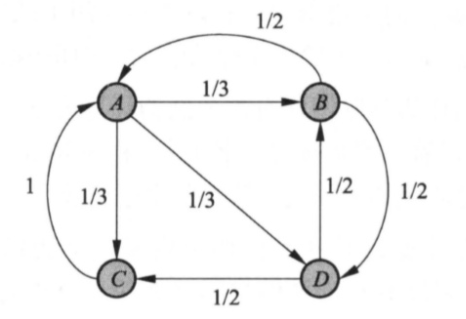
\includegraphics[width=0.42\textwidth]{pr.png}
\end{figure}
\end{frame}

\begin{frame}{Google: PageRank Algorithm}
    \begin{figure}
        \centering
        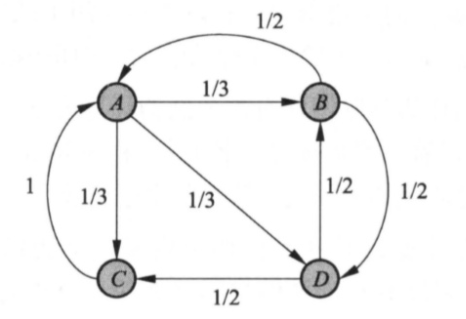
\includegraphics[width=0.45\textwidth]{pr.png}
    \end{figure}

Here is the mathematical model for page ranking. We all know that the web pages always link many other web pages. Just take the simplified case as example, $A,B,C,D$ are all web pages, and the arrows indicate the link.

\vspace{3pt}
\textbf{Assumption:} When the user enter a web page, he will choose one from the links to query next. For example, if a user is currently in web page $A$, the user will choose one from $B,C,D$ to query next with equal probability.
\end{frame}

\begin{frame}{Google: PageRank Algorithm}
Use Matrix to represent the link relations:
\begin{equation*}
    S=\left[ \begin{matrix}
        0&		1/2&		1&		0\\
        1/3&		0&		0&		1/2\\
        1/3&		0&		0&		1/2\\
        1/3&		1/2&		0&		0\\
    \end{matrix} \right]
\end{equation*}

Define the population score: more users enter the webpage, higher score, also higher importance.

\vspace{3pt}
Initialize the population score with all $1/2$.

\end{frame}




\end{document}